\newpage

\section{Versuchsaufbau}
Der allgemeine versuchsaufbau ist in Abb.1 zu sehen. Die zu untersuchende, würfelförmige
Probe ist mit einer Heizwicklung umgeben und mit einem Pt-100-Widerstand verbunden. Die
Heizwicklung hat die aufgabe die Probe zu erwärmen und ist daher an ein Konstantstromgerät
angeschlossen. Der Widerstand ist an ein Ohmmeter angeschlossen, welches ich außerhalb der
Apparatur befindet. Die Proben hängen in einem Kupfer-Zylinder, welcher die Effekte von
auftretender Wärmestrahlung ausgleicht. Um diesen Zylinder ist wieder eine Heizwicklung
angebracht die an eine separaten Stromversorgung angeschlossen ist, zudem ist dort wieder
ein Pt-100-Widerstand angebracht, welcher zu einem
Ohmmeter führt. Dieser Kupfer-Zylinder hängt selbst in dem Rezipenten, welcher einen
Zugang zu einer Vakuumpumpe und einer Helium-Gasflasche besitzt. Zwischen Rezipient und
Heliumflasche befindet sich aus Sicherheitsgründen ein Absperhahn und ein Reduzierventil.
Der Rezipient hängt wiederum in einem Dewar-Gefäß, welches mit flüssigem Stickstoff befüllt
wird. Die einzelnen Komponenten hängen jeweils in einander, da so der Energieaustausch durch
Wärmeleitung unterbunden wird. Das spätere evakuieren schließt zudem den Energieaustausch
durch Konvektion aus.
\begin{figure}[h!]
 \centering
 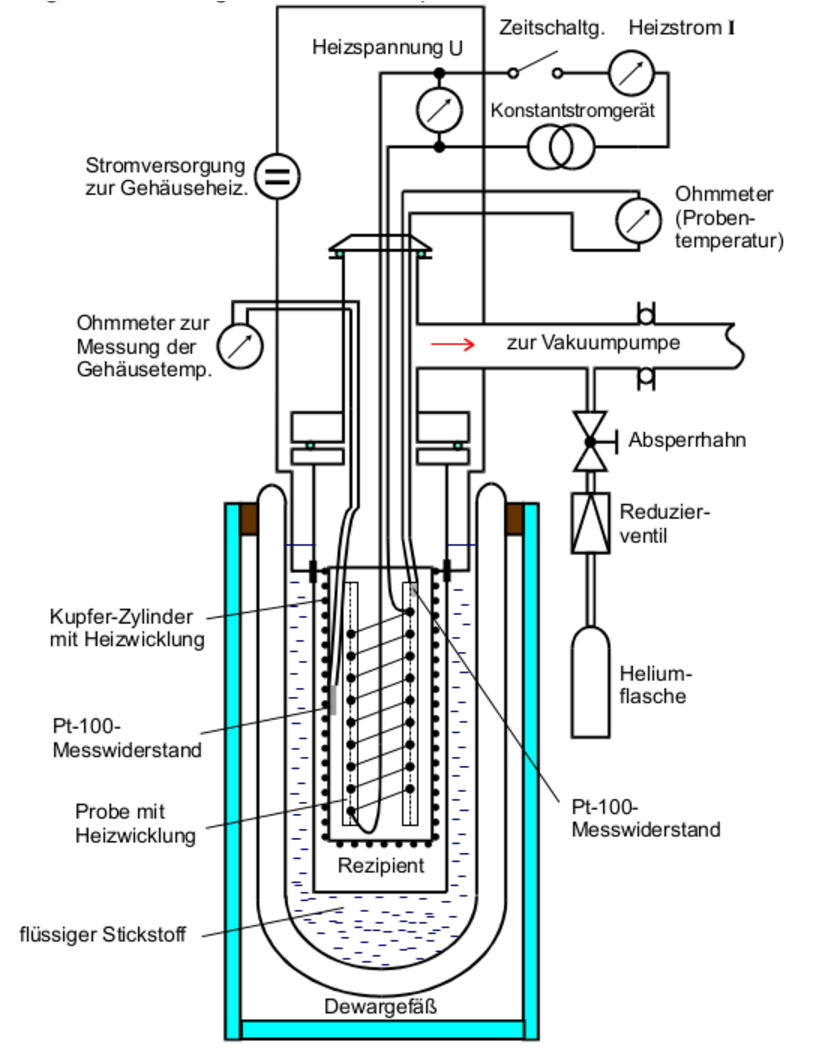
\includegraphics[height=8.0cm]{content/V47.pdf}
 \caption{Aufbau der Messung zur Bestimmung der Molwärme von Festkörpern.}
 \label{fig:Versuchsaufbau1}
\end{figure}
\FloatBarrier

\section{Durchführung}
\label{sec:Durchführung}
Zu Beginn wird der Rezipient evakuiert und mit gasförmigem Helium befüllt.
Dies hat die Aufgabe die Probe und den Rezipient auf selben temperatur zu halten.
Währenddessen wird ständig flüssiger Stickstoff in das Dewar-Gefäß, in dem der Rezipiert
hängt, bis zur Oberkante befüllt. Wenn die Probe auf 80°K abgekühlt ist, schließt
man die Heliumzufuhr und evakuiert den Rezipient erneut. Nun legt man einen
Konstantstrom an der Probe an angelegt. Während der Temperaturunterschied zwischen
Probe und Kupfer-Zylinder bei \SIrange{7}{11}{\kelvin} liegt werden in Abständen von
\SI{10}{\kelvin} die Widerstände der Pt-100-Elemente (aus denen die Temperatur errechnet wird),
sowie das zwischenliegende Zeitintervall erfasst. Dies wiederholt sich im Rahmen von
von \SIrange{80}{300}{\kelvin}.
